% ______________________________________________________________________________
%
%   2DV513 Database Theory -- Assignment 1
%
%   Author:  Jonas Sjöberg
%            Linnaeus University
%            js224eh@student.lnu.se
%            github.com/jonasjberg
%            www.jonasjberg.com
%
%  License:  Creative Commons Attribution 4.0 International (CC BY 4.0)
%            <http://creativecommons.org/licenses/by/4.0/legalcode>
%            See LICENSE.md for additional licensing information.
% ______________________________________________________________________________


\section{Task 1 --- MoviesDB}
Exercise from Fundamentals of Database Systems\cite{2dv513:fds}.

I have used the 7th edition which differs slightly from the 5th edition.
The relevant diagram is included in Figure~\ref{fig:fds_3-25} for reference.


\begin{figure}[htbp]
  \centering
  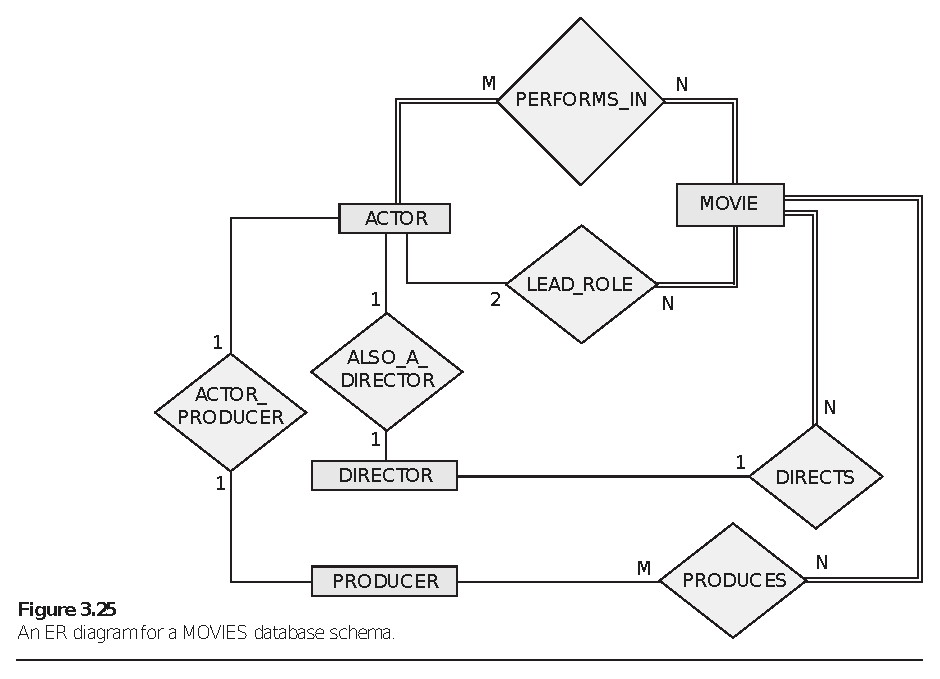
\includegraphics[width=\linewidth]{include/fds_figure_3-25.eps}
	\caption{Diagram from the 7th edition of Fundamentals of Database
           Systems\cite{2dv513:fds}}
  \label{fig:fds_3-25}
\end{figure}


\subsection{Problem Description}
The problem description \cite{2dv513:assignment1-instructions} is stated as
follows:

\begin{quote}
  Assume that MoviesDB is a populated database.

	Given the constraints shown in the E/R diagram,
	respond to the following statements with True, False, or Maybe.

	Assign a response of Maybe to statements that, although not explicitly
  shown to be True, cannot be proven False based on the schema as shown.

  Justify each answer.

  \begin{enumerate}
    \item
      There are no actors in this database that have been in no movies.
    \item
      There are some actors who have acted in more than ten movies.
    \item
      Some actors have done a lead role in multiple movies.
    \item
      A movie can have only a maximum of two lead actors.
    \item
      Every director has been an actor in some movie.
    \item
      No producer has ever been an actor.
    \item
      A producer cannot be an actor in some other movie.
    \item
      There are movies with more than a dozen actors.
    \item
      Some producers have been a director as well.
    \item
      Most movies have one director and one producer.
    \item
      Some movies have one director but several producers.
    \item
      There are some actors who have done a lead role, directed a movie,
      and produced a movie.
    \item
      No movie has a director who also acted in that movie.
  \end{enumerate}
\end{quote}


\subsection{Solutions}

\subsubsection{1 --- There are no actors in this database that have been in no movies}
\textbf{False.} Double lines between \texttt{ACTOR} and \texttt{PERFORMS\_IN}
describe a total participation of \texttt{ACTOR} in the \texttt{PERFORMS\_IN}
relationship to the \texttt{MOVIE} entity.
This essentially means that individuals that have been an actor is considered
an actor.


\subsubsection{2 --- There are some actors who have acted in more than ten movies}
\textbf{Maybe.} The relationship between \texttt{ACTOR} and \texttt{MOVIE} is
many-to-many.  The diagram does not include specific counts.

\subsubsection{3 --- Some actors have done a lead role in multiple movies}
\textbf{Maybe.} The \texttt{LEAD\_ROLE} relationship only specifies a maximum
of \texttt{ACTOR} entities per \texttt{MOVIE}.  There is no minimum
requirement; a movie can have either none, one or two actors in lead roles.
However, all movies must have at least one \texttt{LEAD\_ROLE} relationship,
because of the double lines --- total participation. 


\subsubsection{4 --- A movie can have only a maximum of two lead actors}
\textbf{True.} See above and Figure~\ref{fig:cse_slides_21}
from \cite{2dv513:cse_slides_21}.


\begin{figure}[htbp]
  \centering
  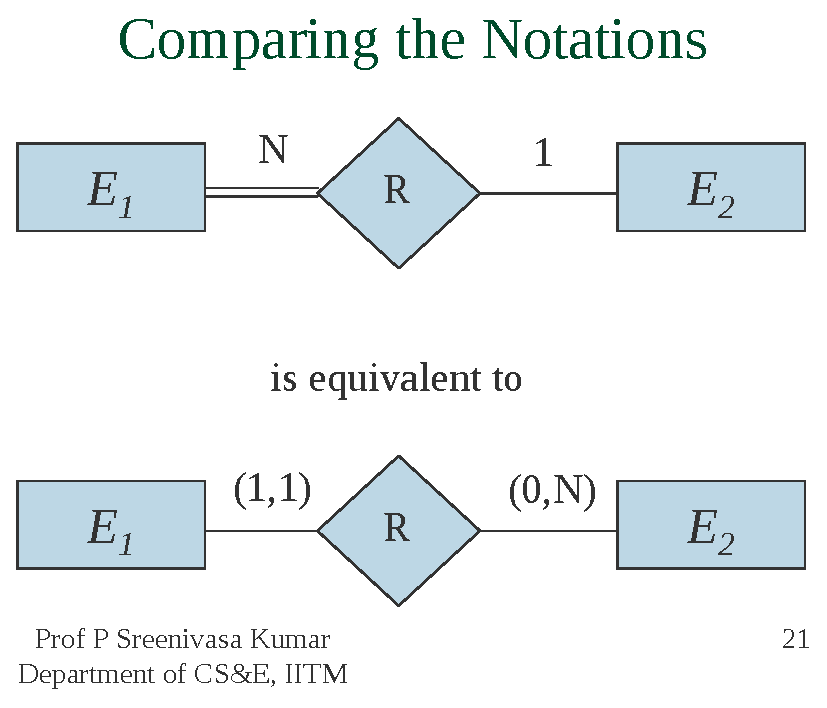
\includegraphics[width=0.6\linewidth]{include/cse_slides_21.eps}
    \caption{Diagram comparing the different notations
             \cite{2dv513:cse_slides_21}}
  \label{fig:cse_slides_21}
\end{figure}


\subsubsection{5 --- Every director has been an actor in some movie}
\textbf{False.} The relationship \texttt{ALSO\_A\_DIRECTOR} is one-to-one,
meaning that an \texttt{ACTOR} entity that is also a director must be
related to one \tettt{DIRECTOR} entity.
An \texttt{ACTOR} must per definition have a \texttt{ALSO\_A\_DIRECTOR}
relationship to \texttt{DIRECTOR} in order to actually be a director,
as far as this system is concerned.

\subsubsection{6 --- No producer has ever been an actor}
\textbf{Maybe.} This might be true, but the diagram only specifies that
\emph{if} an \texttt{ACTOR} was a \texttt{PRODUCER}, it would be a one-to-one
relationship through \texttt{ACTOR\_PRODUCER}.

See the previous motivation. 

\subsubsection{7 --- A producer cannot be an actor in some other movie}
\textbf{False.} There are no such restrictions.
% TODO: Add further motivation..

\subsubsection{8 --- There are movies with more than a dozen actors}
\textbf{Maybe.} This might be true, but the diagram does not include
any such restriction or requirement.

\subsubsection{9 --- Some producers have been a director as well}
\textbf{Maybe.} This might be true. It is \emph{allowed}, but we would have
to query the actual database in order to get this information.

\subsubsection{10 --- Most movies have one director and one producer}
\textbf{Maybe.} This might be true. It is \emph{allowed}, but we would have
to query the actual database in order to get this information.

\subsubsection{11 --- Some movies have one director but several producers}
\textbf{Maybe.} This might be true. It is \emph{allowed}, but we would have
to query the actual database in order to get this information.

\subsubsection{12 --- There are some actors who have done a lead role, directed a movie, and produced a movie}
% TODO: ..

\subsubsection{13 --- No movie has a director who also acted in that movie}
% TODO: ..

